\begin{figure}[tbp]\centering
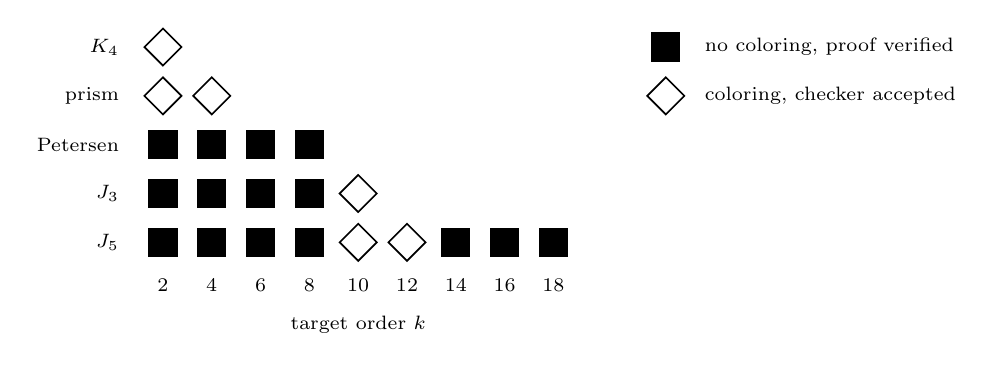
\begin{tikzpicture}[solid, x=0.62cm, y=0.62cm, font=\scriptsize]
\node[anchor=east] at (0.3,0) {$K_4$};
\path[draw, line width=0.6pt] (1.0,0.38) -- (1.38,0) -- (1.0,-0.38) -- (0.62,0) -- cycle;
\node[anchor=east] at (0.3,-1) {prism};
\path[draw, line width=0.6pt] (1.0,-0.62) -- (1.38,-1) -- (1.0,-1.38) -- (0.62,-1) -- cycle;
\path[draw, line width=0.6pt] (2.0,-0.62) -- (2.38,-1) -- (2.0,-1.38) -- (1.62,-1) -- cycle;
\node[anchor=east] at (0.3,-2) {Petersen};
\path[fill=black] (0.7,-2.3) rectangle (1.3,-1.7);
\path[fill=black] (1.7,-2.3) rectangle (2.3,-1.7);
\path[fill=black] (2.7,-2.3) rectangle (3.3,-1.7);
\path[fill=black] (3.7,-2.3) rectangle (4.3,-1.7);
\node[anchor=east] at (0.3,-3) {$J_3$};
\path[fill=black] (0.7,-3.3) rectangle (1.3,-2.7);
\path[fill=black] (1.7,-3.3) rectangle (2.3,-2.7);
\path[fill=black] (2.7,-3.3) rectangle (3.3,-2.7);
\path[fill=black] (3.7,-3.3) rectangle (4.3,-2.7);
\path[draw, line width=0.6pt] (5.0,-2.62) -- (5.38,-3) -- (5.0,-3.38) -- (4.62,-3) -- cycle;
\node[anchor=east] at (0.3,-4) {$J_5$};
\path[fill=black] (0.7,-4.3) rectangle (1.3,-3.7);
\path[fill=black] (1.7,-4.3) rectangle (2.3,-3.7);
\path[fill=black] (2.7,-4.3) rectangle (3.3,-3.7);
\path[fill=black] (3.7,-4.3) rectangle (4.3,-3.7);
\path[draw, line width=0.6pt] (5.0,-3.62) -- (5.38,-4) -- (5.0,-4.38) -- (4.62,-4) -- cycle;
\path[draw, line width=0.6pt] (6.0,-3.62) -- (6.38,-4) -- (6.0,-4.38) -- (5.62,-4) -- cycle;
\path[fill=black] (6.7,-4.3) rectangle (7.3,-3.7);
\path[fill=black] (7.7,-4.3) rectangle (8.3,-3.7);
\path[fill=black] (8.7,-4.3) rectangle (9.3,-3.7);
\node[anchor=north] at (1.0,-4.55) {2};
\node[anchor=north] at (2.0,-4.55) {4};
\node[anchor=north] at (3.0,-4.55) {6};
\node[anchor=north] at (4.0,-4.55) {8};
\node[anchor=north] at (5.0,-4.55) {10};
\node[anchor=north] at (6.0,-4.55) {12};
\node[anchor=north] at (7.0,-4.55) {14};
\node[anchor=north] at (8.0,-4.55) {16};
\node[anchor=north] at (9.0,-4.55) {18};
\node[anchor=north] at (5,-5.3) {target order $k$};
\path[fill=black] (11,-0.3) rectangle (11.6,0.3);
\node[anchor=west] at (11.9,0) {no coloring, proof verified};
\path[draw, line width=0.6pt] (11.3,-1.38) -- (11.68,-1) -- (11.3,-0.62) -- (10.92,-1) -- cycle;
\node[anchor=west] at (11.9,-1) {coloring, checker accepted};
\end{tikzpicture}
\caption{Answers of the 21 control instances of Table~\ref{tab:controls} by graph and target order. The two encodings agree in every cell. The Petersen graph is colored by no graph of smaller order; the flower snark $J_5$ is colored at orders 10 and 12 only, and $J_3$ at order 10 only.}\label{fig:controls}
\end{figure}
